\documentclass[a4paper,10pt]{article}
\usepackage[utf8]{inputenc}
\usepackage{amsmath}
\usepackage{fullpage}
\usepackage{hyperref}
\usepackage{graphicx}
\usepackage{listings}
\usepackage{color}

\definecolor{mygreen}{rgb}{0,0.6,0}
\definecolor{mygray}{rgb}{0.5,0.5,0.5}
\definecolor{mymauve}{rgb}{0.58,0,0.82}

\lstset{ 
  backgroundcolor=\color{white},   % choose the background color; you must add \usepackage{color} or \usepackage{xcolor}; should come as last argument
  basicstyle=\footnotesize,        % the size of the fonts that are used for the code
  breakatwhitespace=false,         % sets if automatic breaks should only happen at whitespace
  breaklines=true,                 % sets automatic line breaking
  captionpos=b,                    % sets the caption-position to bottom
  commentstyle=\color{mygreen},    % comment style
  deletekeywords={...},            % if you want to delete keywords from the given language
  escapeinside={\%*}{*)},          % if you want to add LaTeX within your code
  extendedchars=true,              % lets you use non-ASCII characters; for 8-bits encodings only, does not work with UTF-8
  firstnumber=1,                   % start line enumeration with line 1000
  frame=single,	                   % adds a frame around the code
  keepspaces=true,                 % keeps spaces in text, useful for keeping indentation of code (possibly needs columns=flexible)
  keywordstyle=\color{blue},       % keyword style
  language=Python,                 % the language of the code
  morekeywords={*,...},            % if you want to add more keywords to the set
  numbers=left,                    % where to put the line-numbers; possible values are (none, left, right)
  numbersep=5pt,                   % how far the line-numbers are from the code
  numberstyle=\tiny\color{mygray}, % the style that is used for the line-numbers
  rulecolor=\color{black},         % if not set, the frame-color may be changed on line-breaks within not-black text (e.g. comments (green here))
  showspaces=false,                % show spaces everywhere adding particular underscores; it overrides 'showstringspaces'
  showstringspaces=false,          % underline spaces within strings only
  showtabs=false,                  % show tabs within strings adding particular underscores
  stepnumber=1,                    % the step between two line-numbers. If it's 1, each line will be numbered
  stringstyle=\color{mymauve},     % string literal style
  tabsize=4,	                   % sets default tabsize to 2 spaces
  title=\lstname                   % show the filename of files included with \lstinputlisting; also try caption instead of title
}


\renewenvironment{abstract}
 { \vspace*{0.3cm} \textbf{\abstractname} \vspace{0.1cm} \\ \ignorespaces}
 {\par\medskip \vspace{0.1cm}}

\setlength{\parindent}{0em}

\setlength{\textheight}{25.7cm}
\setlength{\textwidth}{18cm}
\setlength{\unitlength}{1mm}
\setlength{\topskip}{2truecm}

\topmargin 260mm \advance \topmargin -\textheight
\divide \topmargin by 2 \advance \topmargin -1in
\headheight 0pt \headsep 0pt \leftmargin 210mm \advance
\leftmargin -\textwidth
\divide \leftmargin by 2 \advance \leftmargin -1in
\oddsidemargin \leftmargin \evensidemargin \leftmargin
\parindent=0pt
\frenchspacing


%opening
\title{\textbf{Numerical Recipes for Astrophysics \\ Solutions hand-in assignment-2}}
\author{Luther Algra - s1633376}

\begin{document}

\maketitle

\hrule
\begin{abstract}
The current document contains the solutions for the second hand-in assignment of Numerical Recipes. Each main question 1, 2, 3, ..., 7 is given its own section and contains a subsection for each sub-question (1.a, 1.b, ..., 1.f). A main question always ends with a final subsection that contains two segments of code. The first segment contains the full code of the program that executes the sub-questions. The second segment contains the shared modules (if any) used by the sub-question. A sub-question its self always starts with a short summary of the question that needs to be answered followed by an explanation of how the problem is solved. Next, the code and its output are provided. Finally the output is discussed if relevant. 


\end{abstract}
\hrule
\vspace{0.5cm}


\section*{\textbf{1 - Normally distributed pseudo-random numbers} \hrule} 



\subsection*{\textbf{Question 1.a}}
\begin{quote}

\textbf{Problem}
\begin{quote}Write a random number generator that returns a random floating-point number between 0 and 1. At minimum, use some combination of an MWC and a 64-bit XOR-shift. Plot a sequential of random numbers against each other in a scatter plot ($x_{i+1}$ vs $x_{i}$) for the first 1000 numbers generated. Also plot the value of the random numbers for the first 1000 numbers vs the index of the random number, this mean the x-axis has a value from 0 through 999 and the y-axis 0 through 1). Finally, have your code generate 1,000,000 random numbers and plot the result of binning these in 20 bins 0.05 wide. 
\end{quote}

\textbf{Solution} 


\begin{quote}
The state of the random number generator is updated by first performing a 64-bit XOR-shift on the current state and then giving a modified version of the obtained output to the MWC algorithm. The modification of the XOR-shifts output consists of putting the last 32 bits to zero. This is done by performing the 'AND' operation with the maximum value of an unsigned int 32. This modification was performed as the  MWC algorithm expects as input a 64-bit unsigned integer with a value between  $0 < x < 2^{32}$.

The output of the MWC algorithm for this modified value is set as new state of the random number generator. The first 32 bits of the new state are used to provide a random value, as the output of the MWC algorithm only contains 32 significant bits. This random value is obtained by performing the 'AND' operation between the seed and the maximum value of an unsigned int 32. The resulting value is then divided by the maximum value of an uint32 to obtain a value between 0 and 1.

The code for the random number generator can be found at the end of this section, as it is treated as a shared module. The code for generating the plots and the created plots can be found below. 
\end{quote}
\newpage

\textbf{Code - Plots}


% consists of the code that initializes the random number generator and calls the function.

\begin{quote}
The code for generating the plots. The initialization of the created random number generator is not explicitly shown in this piece of code but can be found on page .. where the full code is shown that contains all sub-questions together.

\lstinputlisting[firstline=25,lastline=59]{./Code/assigment1.py}
\end{quote}
\end{quote}

\textbf{Code - Output text } 
\begin{quote}
The text output produced by the code:
\lstinputlisting[firstline=0,lastline=1]{./Output/assigment1_out.txt}
\end{quote}
\newpage

\textbf{Code - Output plots}
\begin{quote}

\begin{figure}[!ht]
\centering
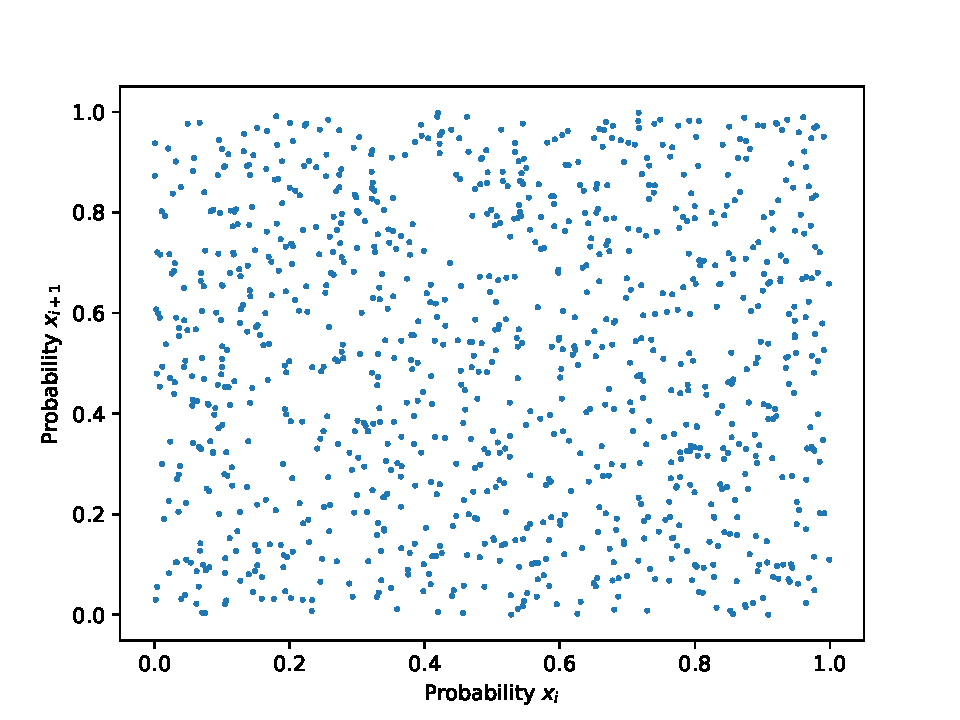
\includegraphics[width=12cm, height=7.5cm]{./Plots/1_plot_against.pdf}
\caption{TODO}
\end{figure}

\begin{figure}[!hb]
\centering
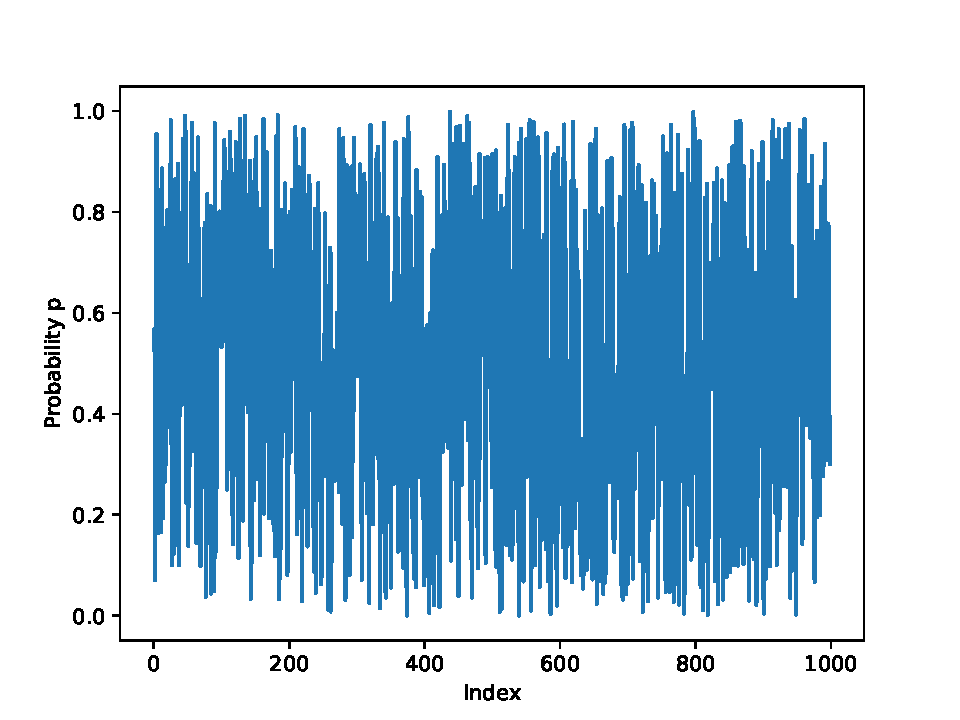
\includegraphics[width=12cm, height=7.5cm]{./Plots/1_plot_index.pdf}
\caption{TODO}
\end{figure}

\newpage
\begin{figure}[!ht]
\centering
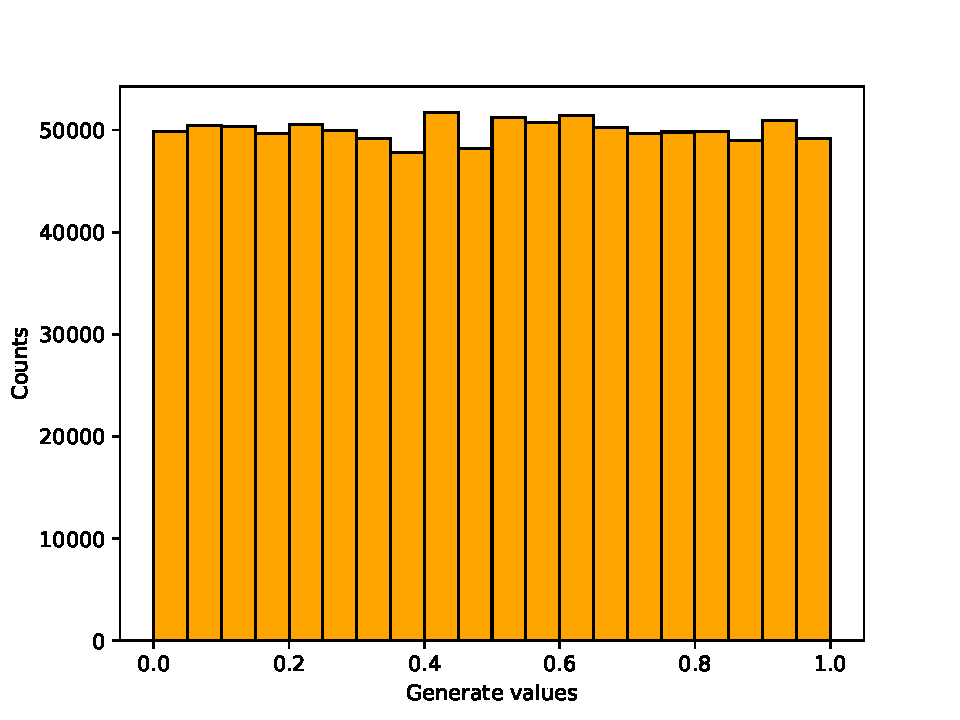
\includegraphics[width=12cm, height=7.5cm]{./Plots/1_hist_uniformnes.pdf}
\caption{TODO}
\end{figure}
\end{quote}


%\textbf{Code - helper } 
%\begin{quote}
%The code for the Poisson distribution and the factorial function.  
%\lstinputlisting[firstline=2,lastline=46]{./code/mathlib/utils.py}
%\end{quote}


%\textbf{Output}
%\begin{quote}
%The output produced by \textsf{/code/assigment1\_ a.py} 
%\lstinputlisting{./output/assigment1_a_out.txt}
%\end{quote}
















  







\end{document}
